\documentclass[12pt]{article}

\usepackage{graphicx}
\usepackage{subfig}
\usepackage{wrapfig}

\setlength{\textheight}{8.5in}
\setlength{\headheight}{.25in}
\setlength{\headsep}{.25in}
\setlength{\topmargin}{0in}
\setlength{\textwidth}{6.5in}
\setlength{\oddsidemargin}{0in}
\setlength{\evensidemargin}{0in}

\title{PartyUp Report}
\author{David Gilhooley, Lance Goodridge, Blake Lawson, and Graham Turk}

\begin{document}

\pagestyle{plain}

\maketitle

\section{Motivation} % (fold)
\label{sec:Motivation}
We created PartyUp to help friends communicate at parties and other events.
We designed the app with the idea that it would allow users to quickly change plans, find where their friends are, and better facilitate party safety.

PartyUp was built to give users an easy way to plan a night out with friends and keep track of those friends throughout the night.
Most social media apps focus on single events or permanent groups, which don't always make sense in a party setting.
PartyUp focuses on groups that are going to a specific event.
Because each group must be tied to at least one event, PartyUp knows when the group should eventually be disbanded.
This gives PartyUp groups the ephemeral quality that is currently enjoyed in apps like Snapchat and Yik Yak.

In other social media apps, it is difficult to adapt to changing plans.
In PartyUp, groups are able to quickly add or create a new event, check on the locations of their group members, and send messages back and forth. This helps the group stay together even when the events around them are changing. 

Party safety is always important, and we we have also taken steps to address this in our app. A group member can quickly see the statuses of the other group members and whether or not they have checked in to the current event. If a user has not checked in, then we can see the last place where the user was going. Single tap `pings' also allow for groups to quickly send notifications to missing group members.
% section Motivation (end)

\section{Design Decisions} % (fold)
\label{sec:design_decisions}

% section design_decisions (end)

\subsection{Front End Design Decisions}

\subsubsection{Design Process}

% picture of index card mockup

\begin{figure}[!htb]
	\centering
	\subfloat[Login and Register Page Mockups] { 
		\includegraphics[width=.628\textwidth]{notecards_1}
	}
	\subfloat[Early My Events Page Mockups] {
		\includegraphics[width=.372\textwidth]{notecards_2}
	}
\end{figure}

In preliminary mockups of PartyUp, we opted for good old-fashioned index cards. Though simplistic, the index cards became some of the most important guidelines when we started to build views in Xcode.
We chose to use Xcode's interface builder tool for all of the UI designs. The tool allows one to drag and drop UI elements onto a canvas, change color schemes visually, and set layout constraints.
Interface builder let us reconstruct the index card UI on a virtual canvas. It gave us a clear picture of the app's aesthetics before it was running on a phone. 
Perhaps even more useful, interface builder facilitates creating outlets and target-action methods between the view and code. 
In what was a bizarre experience at first, you can actually drag from a canvas element directly to the source code to generate an outlet variable or action method. 

\subsubsection{Xcode Challenges}

Despite the usefulness of interface builder, we quickly learned that it is not designed for version control.
Without explicit control over the generated code, we frequently ran into nasty merge conflicts in the XML file.
Looking back, it's tough to say that doing the UI entirely in code would have prevented these merge conflicts. 
Neither of us had experience in Xcode, so programming the UI as well would have been much harder initially. 
However, had we decided to not use the interface builder, we could have saved hours spent inspecting lines of code from merge conflicts in the storyboard file. 

\subsubsection{Swift vs. Objective-C}

We had decided to use the Swift programming language very quickly after beginning the iPhone app development.
Neither members of the front end team had done iOS development, so both Swift and Objective-C would involve learning a new language. 
We feel that Swift is poised to become the dominant iOS language in the future, and it would therefore be the most useful to know if either of us wanted to build another app. 
While reading through the documentation for both languages we saw many similarities between Swift and Python. 
Because everyone had prior Python experience, we saw this as a major plus. 
However, choosing Swift proved to have some significant drawbacks that we did not foresee. 

3 weeks into the project Apple released an update for Swift that broke every file in our front end code base. 
The major update was in how Swift processes Optionals, a structure which handles the absence of a value. 
In Apple's words, ``Optionals say either `there is a value, and it equals x' or `there isn't a value at all'". 
When we originally decided on Swift we had not considered the possibility of a significant language update. 
At the time of the update, it wasn't much of a problem to fix the code. 
However, it alerted us to the fact that Swift is still a new and unstable language. 

With regards to the Swift vs. Objective-C debate, we underestimated the importance of online resources. 
For almost any question we arrived at, there were a bevy of Stack Overflow posts with perfect answers in Objective-C, but barely any in Swift. 
The majority of challenges we faced came from figuring out the CocoaTouch framework, an abstraction layer that handles gesture recognizers and animation, among other UI features. 
CocoaTouch documentation was mostly in Objective-C, so we were sometimes forced to attempt to convert the Objective-C code into Swift. 
Though using Swift came with its problems, the code reads nicely and we hope that learning Swift will be valuable for our futures as developers.

\section{Public API}

One of the best decisions our group made was publishing an api in the backend Github repository. 
The api describes the required post parameter key-value pairs and the contents of the returned JSON file. 
This documentation allows the front end team to quickly look up the required parameters of any backend-interfacing method. 
This meant that the front end team could develop without any back-end members present.
In addition, having the api available opens the door for development in Android or web.

In order for the data from the api to be handled by Xcode the key names of the returned JSON were translated into methods in the data manager class. This class handles all key-value lookups. 

\section{Moving Forward}

The first feature that we would have tried to implement if we had more time is geolocation.
We believe that PartyUp would greatly benefit from using geolocation to find and track group members.
We were originally planning on including this feature, but given our limited time we decided to focus on polishing the app. 
Geolocation would make a lot of the features happen automatically and generally make the app easier to use. 

Another potential extra feature would be an easy way to allow third party event creation and event promotion.
Thinking about the economic potential of an app like PartyUp, we see event promotion as a major source of revenue. 
We would implement this feature as a website, giving local businesses and event organizers the ability to create their event online without having to download the app.

Another feature that still needs to be implemented is front end photo support.
We currently implement photo storage and retrieval on the back end, but the photos are never downloaded and shown in the front end.
This would only take a re-working of the UI to implement the photos.

\section{Challenges}

While building the app, there were a lot of problems that we did not anticipate.
Although we did not find elegant solutions to all of these problems,
there are a couple that stand out that we are proud of.

\subsection{Building the My Groups page}

When it came down to the last week, we realized that the front end team would not be able to complete some of the views we saw as essential to the app. 
The back end team offered to help, but they did not know XCode and they did not have Macs to program on.
We were able to solve both of these problems by writing the views in  HTML, CSS, and JavaScript.
These views were written by the back end and then rendered directly into some of the views. 
We were even able to have it so that the HTML views interfaced with the iOS views directly, through the use of calling certain URLS. 
Though the HTML pages are fully functional, there is a marked difference in look and feel, as well as a short time delay to make the page request. 
Perhaps with an extra week, the front end team would have been able to render these views in iOS and keep a consistent feel across the app. 

\subsection{Group Organization}

When we started working on our project, we did not have a clear strategy for 
delegating work or keeping track of the things that needed to be done.
Initially, we maintained a list of tasks in the Git repository's \texttt{README.md} file,
but we quickly ran into trouble keeping the document up to date.
Furthermore, it was often unclear which people were working on each of the tasks in the README.
There were several occasions in which two people wrote the same function independently
and did not find out until one of them was confronted with a merge conflict when pulling code.
After a few weeks into the project, it was clear that we needed a better system.

\begin{figure}
    \centering
    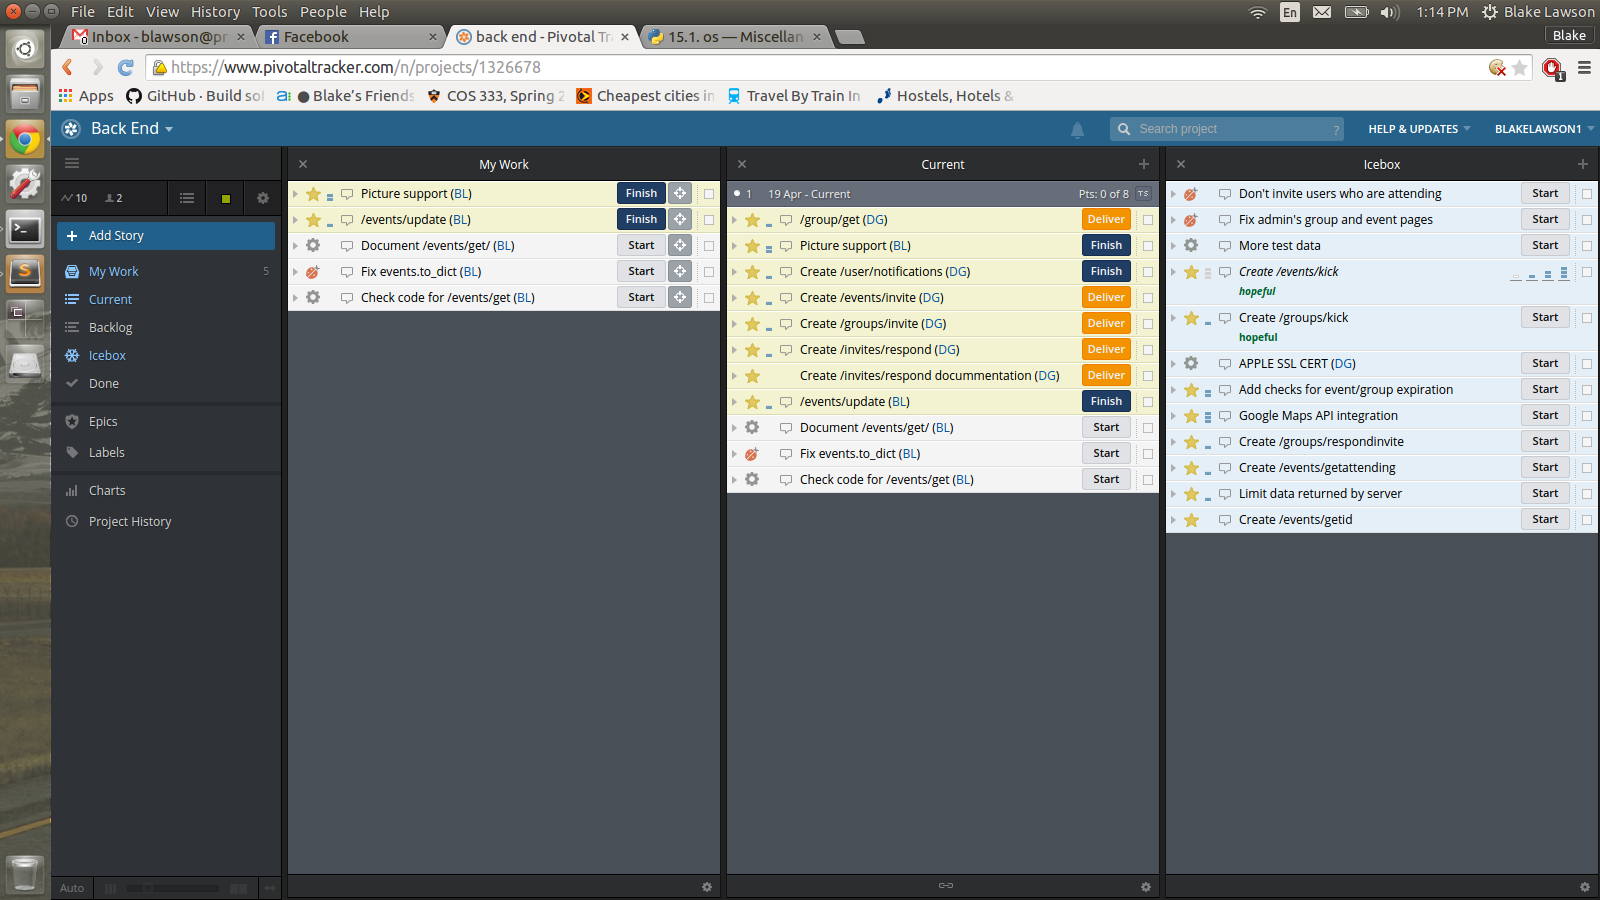
\includegraphics[scale=0.3]{pivotaltracker.png}
    \caption{
        PivotalTracker revolutionized our work flow. 
        This is a picture of the back end's PivotalTracker page around week 4.
    }
    \label{fig:pivotaltracker}
\end{figure}

We decided to try a product called PivotalTracker that we found online,
and we were really happy with the results.
PivotalTracker allowed us to create ``tickets" for each of the tasks that needed to be done.
Group members can then claim tickets so everyone else can see that they are working on it.
Furthermore, PivotalTracker made it easy to add new tasks as we discovered things that needed to be done.
In the end, PivotalTracker saved us a lot of time and make communication and planning way easier.

\subsection{Testing}

A couple weeks into the project, we found that we were making frequent changes to the structure of the database.
Django has a few tools for handling database migrations,
but nevertheless, we had to completely wipe the database a number of times.
At first, we thought that clearing the database wasn't a big deal, but
every time we ran the \texttt{DROP DATABASE partyup;} command,
we needed to repopulate the database with new users, groups, and events,
which took longer and longer as the relationships between the tables got more complicated.

Ultimately, we wrote a Python script that can automatically populate the database with
about 2,000 fake users and a number of fake events.
This script had a few side effects.
On the plus side, it meant that we had a consistent set of test data that made it
possible to automate other tests.
On the other hand, all of those new users exposed a bug in our implementation that we 
probably would not have found otherwise.

The fake user accounts were created from a list of Drexel student emails that
we scraped from their online directory,
and some of those email addresses were quite long.
Problematically, the built-in Django user model that we were using only allowed
user names that were 30 characters or less, and
we were using users' email address as their user name,
which meant that our server crashed every time we tried to create a user with a long email address.
After a few hours of trial and error, we figured out that we could maintain unique user names
by hashing the user's email address and encoding the hash with the base 64 encoding we learned
about earlier in the semester.

We assumed that writing a script to generate test data would be a boring chore--we almost decided not to do
it--but the task exposed a major weakness in our back end and evolved into an interesting technical challenge.

\section{Milestones}

For the first three weeks we stayed right on track with our milestone list. 
We were able to make significant progress at HackPrinceton, which we treated as a feature-thon for PartyUp. 
Login, register, event creation, and group creation were completed on schedule on both the backend and the front end. 
We began to run into difficulties with push notifications and group chat. 
At this point the back end was implementing functions, but there were no views on the front end to implement the features. 
Eventually the back end created the group detail page in HTML to allow the front end to focus on fixing group chat and the other views. 

Almost all of the app's pretty UI was created during reading period, including the currently chosen color theme and fonts. We are very proud of the consistent UI design decisions and we feel that the app is a lot more pleasant to use now.

\section{What we would have done differently}

If we were to start over, I think we would have chosen a narrower problem to address. 
From the demos we attended, the most successful ones were those that performed one well-defined task. 
Although we laid out the target features in our initial design document, there was a lot of leeway and we never had a single, clear direction for the app.
In addition, we would have picked a technology stack that allowed more collaboration between the teams.
An ideal technology stack would allow either the two teams to progress in parallel or one team to help the other in the event of a setback. 
Because the back end had Django experience, the back end team was consistently ahead of the front end.

\section{Advice for next year's class}

To the COS 333 class of 2016, when planning your project, we recommend setting realistic goals. 
Pick a well-defined problem with a baseline solution you know you can finish in around 4 weeks.
Features can always get added on top of the core functionality, but you want to have something you
can proudly present even if all the work does not get finished by demo day.

Without having to turn in something each week, it is easy to put off work until the end of the semester.
However, it is simply not feasible to build a fully functional app in the week before the demo. 
Things will break, and you want leave time for testing and polishing.
It is therefore important to to treat the weekly milestones like they were any regular class assignments, with hard deadlines. 
If you are running behind schedule for multiple weeks, consider dropping a feature.
Beyond that, just have fun with it. It's not every class that you get to build an app with your friends.

\section{Group Reflection}

Building PartyUp was unlike any school project we have ever done. 
We had complete autonomy over the app, a scary notion at first but one that allowed us to develop our creativity. 
In our case, delegation of work was essential; the project was simply too big and too complex for any one person to dominate. 
Two of our group members didn't have Mac computers, so they were completely unable to work on the iOS portion of the code. 
Every one of us had to rely on other people; a feature of any real-world software development project. 
It was difficult for many of the team members to completely trust that features were going to be completed in time, but in the end we were all satisfied with the final project.

\end{document}
